% !TEX root = ./master.tex
\subsection{Technique de passation du test Tomatis}
Nous allons aller plus avant sur le test d'écoute pour plus de détails et de précision sur son utilisation.
L'appareil de Tomatis, basé sur la reconnaissance des sons purs 
%\footnote{Cf. p. 34--35, "L'oreille et le langage" Ed. Points, Science} 
et permettant d'
\enquote{objectiver la qualité de l'écoute} \autocite [34--35]{Tomatislangage}
 a été créé dans les années 50, comportant un générateur de fréquences
  de 125 à 8000 Hz, d'octave en octave, en passant par les valeurs
1500, 3000 et 6000 Hz, et dont l'intensité peut varier de 5 en \SI{5}{\dB}, de 10 à 100 dB.
Les sons purs sont émis par 
  transmission aérienne avec un casque, et par transmission osseuse
  avec un vibrateur.
L'identification de ces sons est
  signalée par la levée de la main homo-latérale (droite, gauche ou
  bilatérale).
Un volume initial très faible est suivi d'une intensité
progressivement plus élevée jusqu'à la manifestation d'une réponse gestuelle.

%Nous allons développer à l'aide de la représentation
%graphique de la courbe idéale (Fig 3. 5) les paramètres du\textbf{ seuil}, de la
%\textbf{spatialisation}, de la \textbf{sélectivité} et de l'\textbf{au\-dio\-latérométrie}.


\begin{figure}
	\centering
	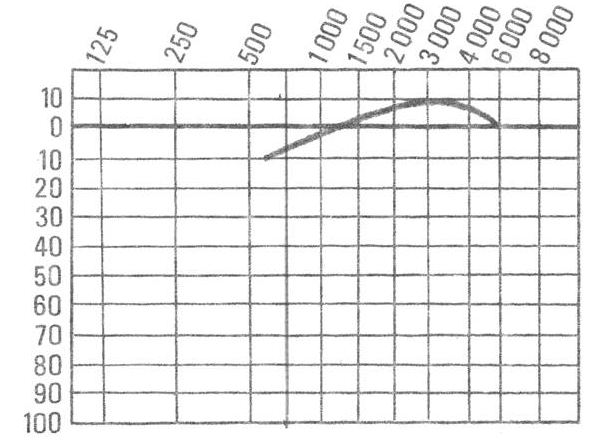
\includegraphics[width=1\linewidth]{images/graphiques/courbeideale.png}
	\caption[Courbe idéale]{Diagrammes des courbes relatives à l'oreille droite et
          gauche; tracé bleu: c. aérienne; tracé rouge: c.
          osseuse, (Copyrights Tomatis Développement S.A.  2014) }
	\label{Courbe idéale}
\end{figure}




\paragraph{Identification des seuils auditifs individuels et représentation graphique}

Cette \textbf{détection}, destinée à révéler les deux profils d'écoute
s'effectue, d'une part, à l'aide d'une
conduction aérienne par \textbf{écouteurs}, où l'oreille interne
informe le nerf auditif,  et d'autre part, à l'aide
d'une conduction osseuse par\textbf{ vibrateur}, excitant le crâne au
niveau de l'
\textit{os mastoïde} transmettant à son tour à  la voie nerveuse
auditive.
Parmi les quelques éléments différentiels
apparaissant par la suite dans les observations cliniques, il est utile de retenir
que le \textbf{seuil d'écoute} est représenté par un point, résultant entre la
fréquence (abscisse) --spectre couvrant 20
fréquences (de 125 à 8000 Hz)--   et le volume
(ordonnée) dont chaque carré représente une différence de \SI{5}{\dB} en
volume, partant de dB de $-20$ à 90 dB.
Les points reliés dessinent deux courbes caractéristiques, aérienne
et osseuse, permettant de relever les paramètres d'harmonie ou
          d'équilibre, ceci
 	en comparaison avec la courbe idéale : on parlera
        d'équilibre ou de
 	déséquilibre, d'harmonie ou de dysharmonie. 	
 	
En résumé: 
        \begin{enumerate}

  \item   Les seuils d'écoute sont reconnaissables par des points au niveau de
          chaque fréquence émise et selon le volume entendu par le
          patient. Les points reliés créent les deux courbes.
 	\item Le son : son pur en 20 fréquences différentes, de 125 à 8000 Hz.
 	\item Le volume: dB de $-20$ à 90; un carré sur le graphique représente une différence de \SI{5}{\dB} en
 		volume
 	\item La courbe: est le résultat des points reliés des seuils
          d'écoute; ils
          dessinent deux courbes caractéristiques, l'une aérienne et l'autre osseuse.
\item L'équilibre/déséquilibre graphique s'observe
        -entre les deux oreilles, l'oreille droite et l'oreille gauche
        et
        -entre les deux courbes aériennes et osseuses, dont les
        croisements, les pics ou les échancrures représentent
        l'écart en
        qualifiant l'écoute d'harmonieuse ou de
        déséquilibrée.
      \end{enumerate}

 En  conséquence,  s'il y a une modification
          graphique des courbes, elle
          permettra de constater s'il y a \textbf{une transformation de l'écoute}
          et l'évaluer pré -- et
          post -- thérapie.




Soulignons que Tomatis a volontairement décalé les étalonnages des deux courbes (aérienne et osseuse) pour pouvoir distinguer les différentes réponses et interpréter
	les \textbf{distorsions}. Lorsque l'écoute est harmonieuse, les
	courbes aérienne et osseuse se confondent mais pour l'analyse des
	résultats, on a déterminé des courbes parallèles, la courbe aérienne
	devant être au dessus de la courbe osseuse.


\begin{figure}
	\centering
	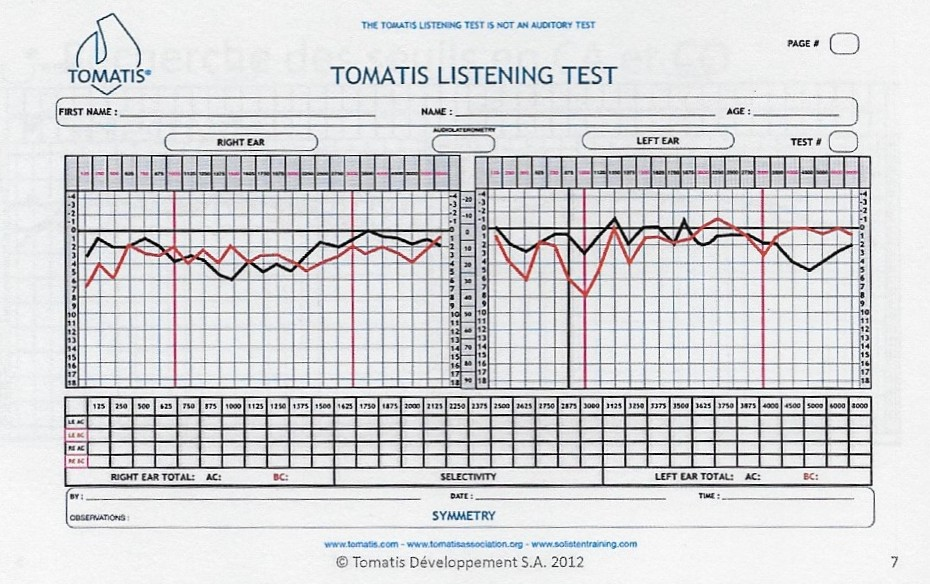
\includegraphics[width=1\linewidth]{images/tomatisListeningTest.jpg}
	\caption[Test d'écoute]{Test
          d'écoute asymétrique des deux oreilles}
	\label{Test d'écoute asymétrique avec oreille droite et oreille gauche}
\end{figure}
%Nous énumèrerons brièvement les
%mentionnées car importantes.
 Il serait intéressant d'englober ici tous les paramètres de la méthode Tomatis et différentes techniques 
 d'observation telles la \textbf{spatialisation, la sélectivité et l'audiolatérométrie}. 
 %mais la complexité d'interprétation de ceux-ci ne concernerait que les 
 %	consultants 
 %	Tomatis et mettrait hors de portée l'analyse pouvant être faite par les musicothérapeutes. 
%  L'objectif de notre travail serait alors largement dépassé.
%Vu sous le très riche angle d'observation de la transformation de l'écoute, 
Nous
donnerons ici la priorité, avec les  \textbf{croisements}, à la comparaison graphique
des courbes aérienne et osseuse, appuyée  par les résultats
% quantitatifs
des \textbf{seuils auditifs} --- en référence à
  l'étude effectuée par le CNRS de Montpellier\autocite{affectiveDisorders} ---.
%\subsection{La spatialisation}
%En relevant les seuils, on assiste à la capacité
%d'\textbf{identification} et de \textbf{localisation} de la
%\textbf{source sonore} comportant parfois des confusions et/ou des inversions
%latérales.
%La \textbf{spatialisation}
%indique le degré d'élaboration de la latéralité auditive,
%et elle fournit des repères sur la façon dont le cortex intègre les informations
%par les faisceaux homo et hétéro -- latéraux fonctionnellement différenciés.
%Selon Tomatis, les erreurs de spatialisation peuvent refléter cette confusion des informations et traduire 
%une latence/
%incertitude de localisation de la provenance du son, difficulté due à une mauvaise coordination.
%\subsection{La sélectivité}
 % La \textbf{sélectivité }s'assimile  à  la CAT, capacité d'analyse tonale, \textquote{faculté que possède 
 %une oreille de percevoir
%une variation de fréquences à l'intérieur d'un spectre sonore, et
%de situer le sens de cette variation}\autocite{tomatis:loreille} dont
%le but est de déceler l'ouverture ou la fermeture de cette
%caractéristique auditive.
%La sélectivité permet de donner des informations sur la
%qualité d'écoute. Elle touche aux aspects  linguistiques (conscience
%phonémique), cognitifs (fonctions exécutives) et émotionnels (action
%efférente, présence d'anxiété).
%Le langage étant lui-même constitué de milliers de phonèmes, Tomatis reconnaît les possibilités 
%%%auditives du patient si celui-ci  distingue au minimum la différence d'un son ``pur" \footnote{Cf. 
%%%%Annexe A. 1. } d'une octave à l'autre.
%\subsection{ L'audiolatérométrie}
%Grâce à l'\textbf{audiolatérométrie}, on définit  la latéralité droite ou gauche du patient. La dominance
%de l'oreille droite comme oreille directrice doit être manifeste car
%selon ses travaux, il y a une différenciation fonctionnelle
%physiologique due à la longueur des nerfs récurrents.
%Si le cerveau préfère prendre l'oreille droite comme
%``directrice'', c'est que le trajet emprunté par l'oreille droite au cerveau est plus
%court; ainsi les informations circulent plus rapidement jusqu'à l'hémisphère gauche.


 \textbf{Par conséquent,} après la passation du test d\textquoteright écoute, nous nous
trouvons en présence de deux grilles, une  pour chaque oreille, contenant deux courbes
de couleurs différentes, permettant de faire une comparaison avec la courbe
 idéale, dite de \textit{Caruso}.
%complétées par l'indication
%des inversions ou confusions de sons, par des données sur la sélectivité
%et en même temps par des chiffres qui correspondent à l'épreuve d'audiolatérométrie.
%Les résultats du test permettront de faire une comparaison avec la
%courbe dénommée idéale\footnote{Cf.\textit{ Caruso } Ch. 3. 1.)}.

  
  
  
  

\paragraph{Analyse et interprétation du test}
De manière générale, l'interprétation du test insiste sur le relevé graphique
des
courbes. Elles donnent des informations selon leur ascendance, leur
continuité et leur similarité oreille droite/ oreille gauche.
%et accorde des
%significations différentes aux zones spectrales.
On considère d'abord l'\textbf{allure }générale des courbes,
% leur
%\textbf{dessin} et la \textbf{forme},
 l' équilibre visuel entre elles et leur symétrie.
Puis on estime
leur\textbf{ rapport} entre eux -- entre la courbe aérienne (CA) -- et la courbe osseuse (CO),
pour chaque oreille ainsi que le rapport entre CA et CO d\textquoteright une
oreille à l'autre. Si ce rapport est correct, CA est placée au-dessus
de CO sur la grille.
Chacune  véhicule des informations spécifiques
sur la posture d'écoute du sujet :
\begin{itemize}
\item La conduction aérienne : traduit la vie sociale, la manière de communiquer
et de s'extérioriser.
\item La conduction osseuse : traduit la vie intérieure, mode de fonctionnement
organique, d'une façon générale : liée aux tensions. C'est la courbe
de l\textquoteright auto-écoute, de l\textquoteright auto-contrôle,
de l'écoute intérieure.
\end{itemize}

Une courbe est définie comme \textbf{harmonieuse}\footnote{Cf. Ch. 1. 2. / 3.1.}
si elle ne comporte pas de
pics, de scotomes
qui laisseraient
supposer l'existence de nombreuse tensions.
Situées en CO, ce sont des tensions internes non exprimées : attitude
calme mais très tendue intérieurement.
Situées en CA, ce sont des tensions réelles et exprimées au quotidien
: soit somatisées, verbalisées ou manifestées sur le plan
affectif, par exemple avec des pleurs.

\paragraph{Les trois zones du test d'écoute et leur interprétation}
Sur le graphique du test, les fréquences observées vont être partagées en
trois zones à l\textquoteright intérieur
de chaque diagramme. Les fréquences se répartissent des
graves aux aigües:
\begin{itemize}
	\item Zone 1 : de 125 à 1000 Hz : les graves, la zone vestibulaire correspondant à l'élaboration
	du schéma corporel, des repères temporo-spatiaux et habiletés motrices; 
	esprit pratique.
	\item Zone 2 : de 1000 à 3000 Hz : les mediums, correspondant à  la zone du langage, de la
	verbalisation, compréhension, %(Wernicke),
	mémorisation %(Papez), 
	et intégration des lois/
	des règles; esprit analytique.
	%lobes frontaux,
	\item Zone 3 : de 3000 à 8000 Hz : les aigus, la zone cochléaire, correspondant à l'énergie,
	 l'imagination, à l'expression, et à la motivation; esprit synthétique.
%	fonctions de survie, pulsion à l'état primitif, cortex
	%hautement spécialisé), 
	
\end{itemize}
Ces trois différentes bandes de fréquences sonores nous donnent des éléments, résultats des   
recherches de Tomatis dans le domaine
empirique. 
%d'interprétation recueillis lors des formations suivies.
%\begin{itemize}
		%\item Zone 1 : de 125 à 1000 Hz : les graves, la zone vestibulaire
	%\item Zone 2 : de 1000 à 3000 Hz : les mediums, la zone du langage
%	\item Zone 3 : de 3000 à 8000 Hz : les aigus, zone cochléaire
%\end{itemize}
%sur les affirmations expérimentales de Tomatis. 
%\paragraph{Interprétation des trois zones du test d'écoute : }
%Les trois zones de fréquences du test d'écoute correspondent à des
%caractéristiques précises ; et, avec l'allure des courbes, on doit
%tenir compte de leurs particularités.
%\textbf{Remarque:} dans le travail qui va suivre, l'allure générale des courbes, le relevé quantitatif des
%  croisements et des seuils auditifs seront notre priorité pour
%  extraire nos résultats à partir de ces tests.
%Nous disposons à présent d'une somme suffisante de renseignements pour
%aborder le chapitre consacré à l'étude clinique.
% et
%l'illustrer par des exemples.


% nous approfond
%aspect par une  description de séances en musicothérapie accompagné des tests d'écoute d'un patient 
%intégré dans cette étude, en détaillant l'impact
%des\textbf{ trois zones} dudit test ainsi que  leur corrélation musicothérapeutique.
%\footnote{ Ces données interprétatives sont fiables, confirmées par
% les recherches de Tomatis dans le domaine
%empirique.}
\begin{figure}
	\centering
	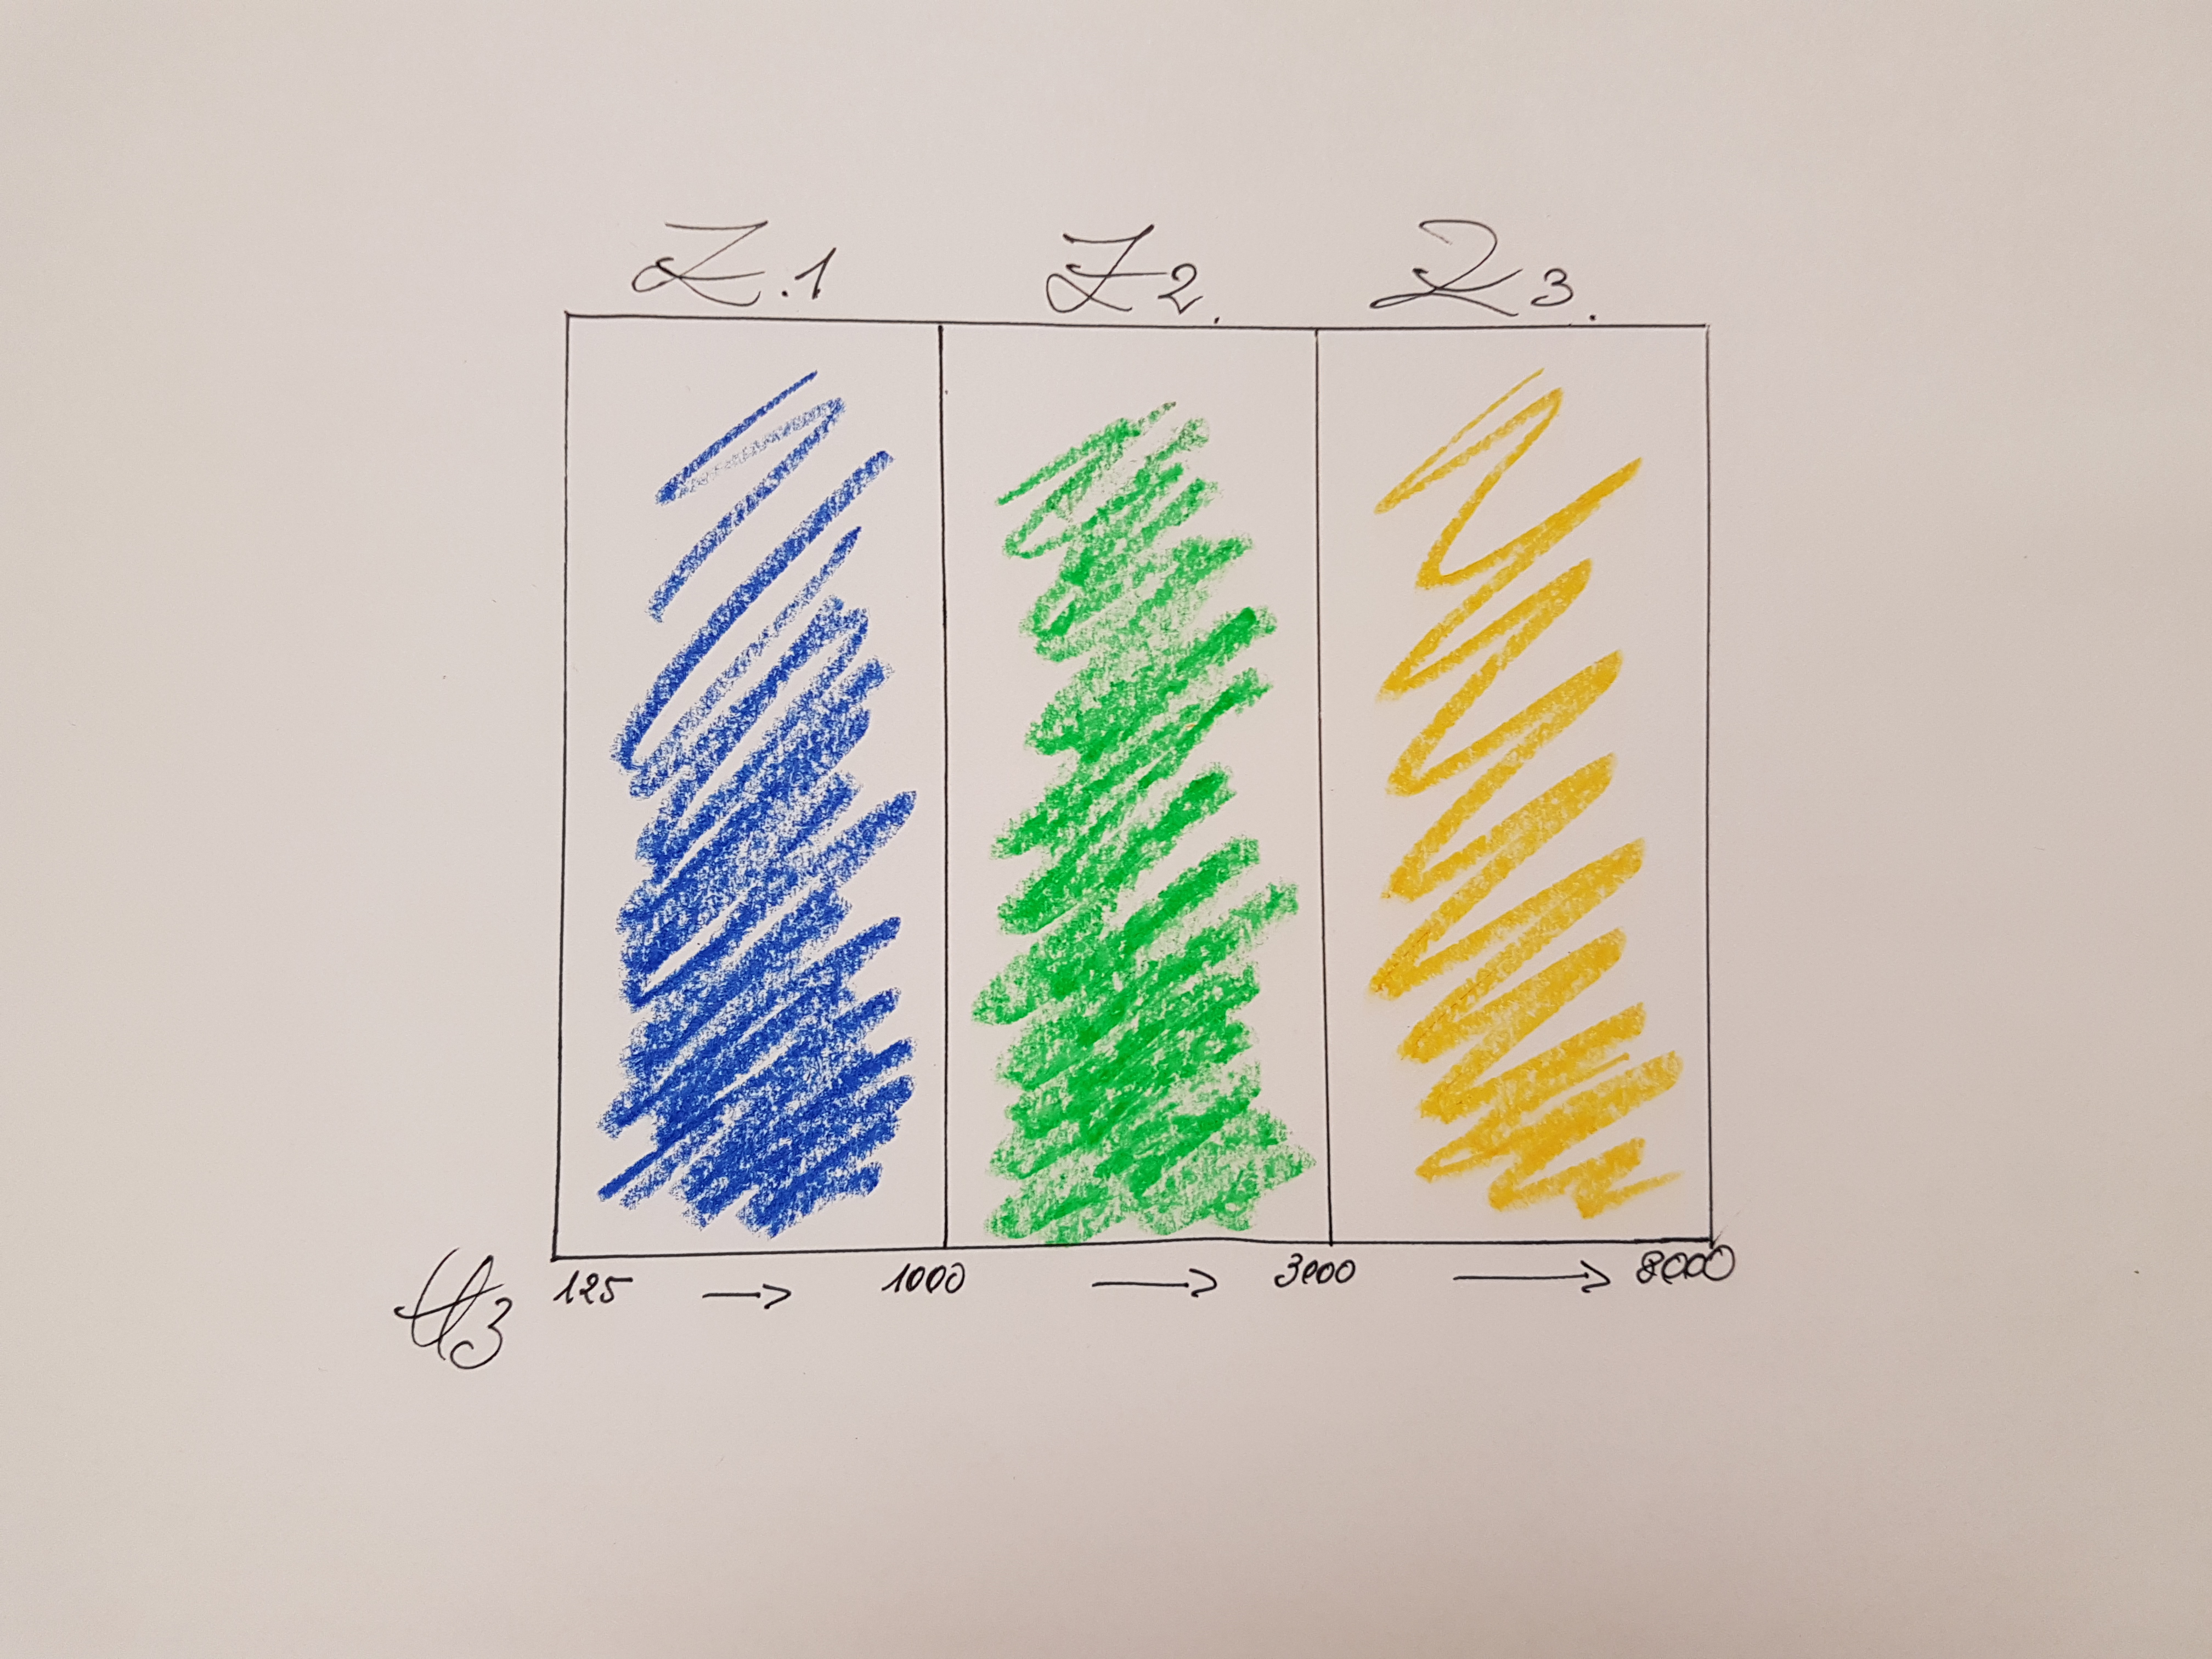
\includegraphics[width=1\linewidth]{images/les3zones.jpg}
	\caption[Les 3 zones]{Les 3 zones}
	\label{Les trois zones du test d'écoute}
\end{figure}
 \clearpage

\subsection{Liens entre test d'écoute, voix et 
humeur négative:}
De manière générale, nous allons passer  à  des considérations et liens entre test d'écoute, voix  et 
humeur négative.


\textbf{Les troubles de l'humeur et leur expression
	musico-phy\-sico-psy\-cho\-lo\-gi\-que:} par le lien entre les troubles
émotionnels et le
système sensoriel, notamment au niveau du cortex auditif, nous
pouvons dresser un portrait
physico-psychologique de ce type de population,
en le mettant en correspondance avec les zones du test d'écoute et
en y ajoutant quelques remarques sur les modifications vocales.
Le test d'écoute ci-dessous fait en clinique lors de notre travail,  illustre
celui d'un sujet diagnostiqué dépressif avec la
chute  de hautes fréquences 
clairement visible dans la troisième zone. Elle correspond au rapport de l'émission du son à
très faible intensité perçue par le
patient, autrement dit à une augmentation
du volume
par le thérapeute jusqu'à ce que le patient les entende et les signale.
Ce sont ses seuils minima de fréquences.


\begin{figure}[ht]
	\centering
	\includegraphics[width=1\linewidth]{images/courbesdeepressif.jpg}
	\caption{Test d'écoute avec troubles de l'humeur}
	\label{fig:courbes du dépressif}
\end{figure}


\paragraph{Descriptif selon les zones d'nterprétation:}

\begin{itemize}
	\item Zone 1 :  Le rythme cardiaque: un stress intense va modifier le rythme
	du corps en augmentant ses fréquences. La respiration deviendra
	rapide. Il va s'en suivre une modification des perceptions
	extérieures. Une sensibilité particulièrement accrue aux bruits et
	aux sons peut en découler et être vécue comme une
	atteinte physique et psychique insupportable.
	Le changement de posture et d'attitude corporelle sont
	notables (affaissement) et la perte d'énergie physique considérable (épuisement).
	\item Zone 2: La qualité de la voix: changement de la qualité du timbre de la
	voix et de l'émission verbale.
	La voix se caractérise par son volume, son timbre, sa mélodie et son
	langage. Nous pouvons en faire le
	descriptif général, rejoignant ainsi l'idée émise lors du Congrès de la Société
	américaine d'acoustique \autocite{le_service_metronews}
	%https://www.lci.fr/sante/et-si-on-diagnostiquait-la-depression-avec-u
	%n-test-vocal-sur-smartphone-1562728.html,
	de diagnostiquer la
	dépression par la voix:\footnote{Maryland University, 2004, 168\ieme\ Congrès de la Société
		américaine d'acoustique.}
		\begin{enumerate}
		\item le volume : basse intensité, faible dynamique
		\item la mélodie : monotone, sans modulation
		\item le timbre : mauvaise qualité due à une pertes des harmoniques
		\item le langage : difficulté d'élocution, manque de fluidité
	\end{enumerate}
	Il en découle une communication difficile avec l'entourage qui
	conduit au retrait social et à l'enfermement sur soi.
	
	De même, un analyseur vocal peut permettre de suivre précisément l'amélioration de
	l'identité vocale; sa visualisation conforte les progrès grâce aux
	formants. L'enveloppe spectrale montre le timbre plus ou moins riche
	dans l'empreinte vocale, renseignements précieux selon les cas.
	
	\item Zone 3: La confusion mentale, la démotivation, la perte d'énergie
	psychique, la disharmonie intérieure/extérieure va provoquer un retrait social sous forme de 
	non-verbalisation ou de mutisme.
\end{itemize}


\subsection{Résonance entre test d'écoute, musicothérapie et
	psychologie}
L'existence de difficultés de perception dans les zones nous
	induit à une meilleure compréhension et  élucidation de ces dernières à l'aide du
	test d'écoute. 
	
	Pour une optimalisation de l'écoute différenciée, afin de s'ajuster à la \textbf{capacité 
	d'écoute de base} 
du patient, on peut suggérer d'adapter et de moduler le \textbf{volume} sonore selon \textbf{les seuils 
d'écoute}. Cet accordement peut passer par 
l'utilisation 
de la voix, \textbf{la zone 2} en musicothérapie.
%de rejoindre dans un premier temps  le patient dans sa \textbf{ capacité
%d'écoute de base}
%avec une adaptation et modulation consécutive du
%  \textbf{volume } sonore selon \textbf{ les seuils auditifs } et, par exemple, de l'utilisation de la voix, 
%\textbf{ la zone 2}, en musicothérapie.
Pour élargir le concept de \textbf{la zone 3,} nous pourrions
également y intégrer les notions winnicottiennes du jeu, de la capacité
créative dans un espace
intermédiaire, où l' \textit{``objet
	transitionnel'' } de D. Winnicott dans \textit{``Jeu et Réalité''}
\autocite{winnicott}
figure entre le ``le
dedans et le
dehors'',
l'interne et l'externe, et, de là, prolonger le questionnement du
rapport avec le concept des
courbes aérienne et osseuse.
De même, si on considère que ``\emph{l'alliage indissociable du corps et du psychisme,
	visible et lisible résulte de l'écoute de
	sons'''}\autocite{tomatis_conf1972}
%\footnote{\emph{Extrait de l'entretien Tomatis réalisé par
%		Auriol, Anvers 1973}},
	 le concept de dépression (R. Jouvent) \autocite{doronparot}  inclut aussi l'idée d'une protection et 
	 une stratégie de
défense du psychisme, ayant un lien évident avec les zones du schéma d'écoute.
Chez E. Willems \autocite{willems} 
%\footnote{\textit{Philosophie de la méthode} issu de sa
%	Pédagogie musicale, Copyright by Musique et Culture, Strasbourg}, 
on relève aussi des correspondances 
	analogues entre les vies
corporelle (impulsions physiques)
--- rythmique, affective (affection et sentiment) --- mélodique, mentale
(raisonnement et intellect) --- harmonique.
     De plus, nous pouvons également nous référer, comme B. Auriol le suggère, à la conception indienne 
     antique des chakras
ainsi qu'au sens de la seconde
topique de Freud (\textit{ça, moi et surmoi}), pour trouver des correspondances
entre les trois zones de
fréquences et \textit {``la distribution de l'énergie pulsionnelle''} ou entre
les
\textit{``caractéristiques du son et l'énergie
	instinctuelle''}\autocite[ch. 13]{auriol:cle}.
\begin{itemize}
	\item  Z.1: le physique, le corps, l'incorporation et
	l'intégration du rythme,
	la posture d'écoute  =  rythme, tempo, puls
	\item  Z.2:  l'expression vocale, la communication,
	l'émotionnel, la sensibilité, l'affect = voix, timbre, mélodie
	\item Z.3: la créativité, l'interprétation, la
	résonance, la musicalité, la motivation, le non-verbal (l'intraduisible en mots), l'espace = justesse, 
	harmonie (consonance,
	dissonance), improvisation.
	%\footnote{\{Hegi : L'improvisation joue un rôle centrale en musicothérapie (Hegi 1986)}
\end{itemize}

Notre recherche nous a mis en évidence ce lien que nous pouvons faire entre 
\textbf{ les trois zones du
	test d'écoute avec des données musicothérapeutiques et des associations psychologiques},  
	suggestions dans une perspective d'analyse 
plus
poussée.
%Nous avons aussi mis
%en parallèle des suggestions d'utilisation d'instruments,(Cf. Annexe A. 10 Fig. A. 4)
%indicateur éventuel des zones de fréquences à
%privilégier.
%Chaque instrument a une tessiture
%différente avec une plage
%définie de fréquences. Selon l'analyse de l'écoute du patient, le choix
%d'instrument à privilégier sera plus rapide et plus sûr.
\begin{figure}
	\centering
%	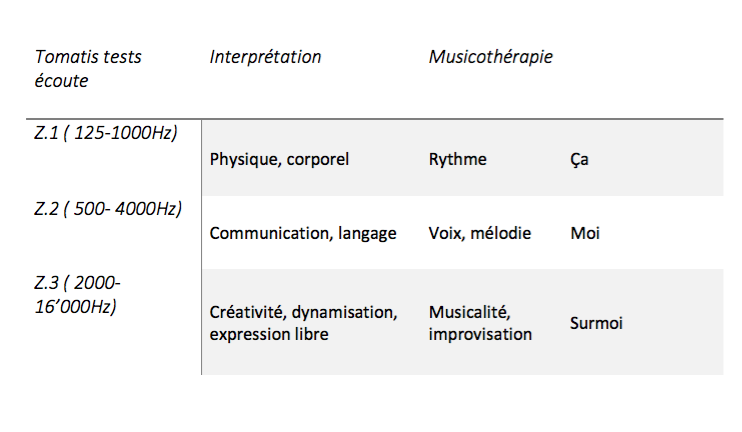
\includegraphics[width=1.1\linewidth]{images/testinterpmusico}
	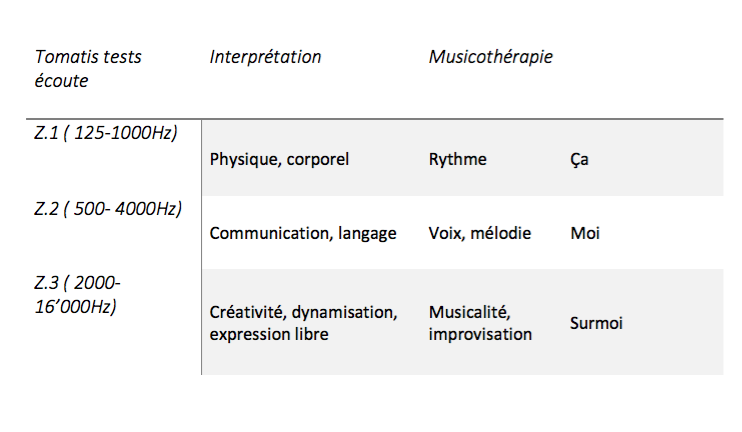
\includegraphics[width=1.0\linewidth]{images/testinterpmusico}
	\caption[ L'interprétation des 3 zones et leur correspondance
	en musicothérapie]{Graphique: interprétation des 3 zones du
		test, leur correspondance en musicothérapie et selon les
		topiques de Freud.}
	
	\label{graphiquecolonnetestmusico}
\end{figure}
 \clearpage
\begin{figure}[tbh]
	\centering
%	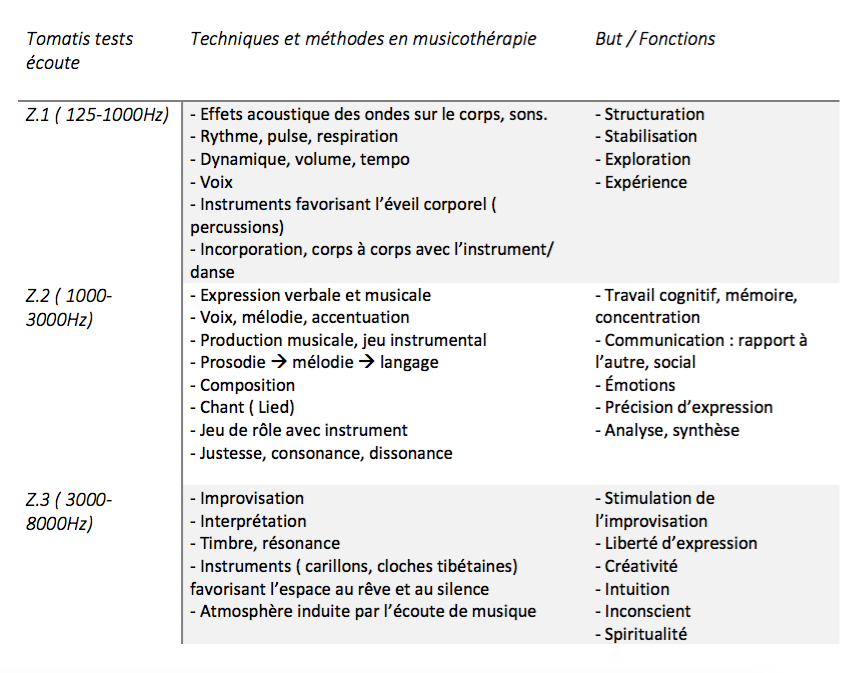
\includegraphics[width=1.2\linewidth]{images/testtechnmethbut}
	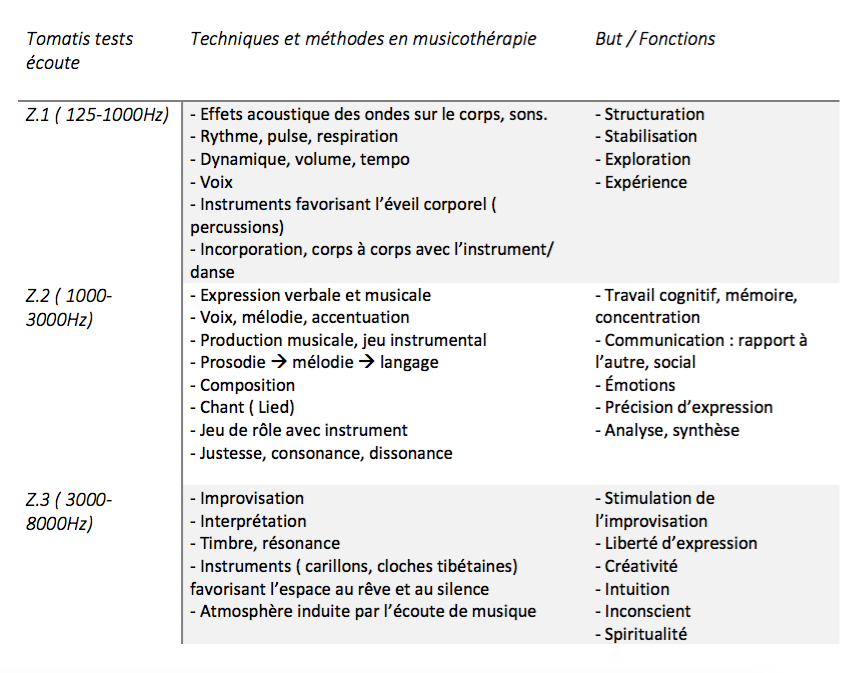
\includegraphics[width=1.0\linewidth]{images/testtechnmethbut}
	\caption[Zones du test avec la musicothérapie]{Les 3
		zones et la musicothérapie}
	
	\label{testbutetfonction}
\end{figure}

Lors du déroulement de l'étude avec les patients que nous allons aborder plus loin, les séances 
de
musicothérapie n'ont pas été
décortiquées dans le but d'analyser les techniques pour différencier de manière systématique  leur  
impact sur la 
modification de 
l'écoute.
%C'eût été passionnant de le faire mais ici, ce n'était pas notre objectif.
Néanmoins, nous  complétons ici ce travail par l'exemple concret d'une  séance de
musicothérapie  avec test d'écoute  d'un 
patient M. du groupe expérimental, réalisée lors de l'Etude clinique.

 \clearpage



\section{ Une séance de musicothérapie avec tests d'écoute}

Avant de rentrer dans le chapitre de la Méthodologie ainsi que celui de l'Etude clinique, nous avons 
choisi de vous présenter,  afin de donner tout de suite un aperçu plus concret  de notre façon de 
procéder, un exemple de 
séance avec le 
patient M. réalisé durant cette 
période, accompagné des tests d'écoute, en détaillant 
l'impact
des\textbf{ trois zones} dudit test ainsi que  leur corrélation musicothérapeutique. Comme nous le 
verrons plus tard, à la différence des 
autres tests d'écoute où on observe le résultat de la moyenne des deux oreilles, nous examinerons 
l'oreille droite.
Nous avons résumé ici le déroulement de deux séances de
musicothérapie d'une durée chacune  de 50 mn,  accompagnées des tests d'écoute --  
schématisés ici  par ordinateur pour une meilleure 
distinction graphique des courbes ---. Ces séances ont eu lieu, comme pour les autres cas 
présentés, dans la Clinique privée de Meiringen en langue allemande et sont rapportées de
manière indépendante du reste de l'étude car elles ne sont pas
suffisamment représentatives.

\textbf{Patient M:}
%Données amnamestiques: âge, profession, famille etc., raison d'hospitalisation
\textbf{ Test d'écoute pré -- musicothérapie:}
Le patient, un homme de 35 ans, manager,  est venu en clinique en raison d'un burnout, déclenché par 
une maltraitance psychologique. Effondré et nerveux, il  se montre curieux et 
intéressé pour participer à l'étude. Nous allons faire
l'observation plus attentive de
son oreille droite, l'oreille ``directrice'',
celle qui est la plus perturbée dans son cas.


\begin{figure}[tbh]
	\centering
	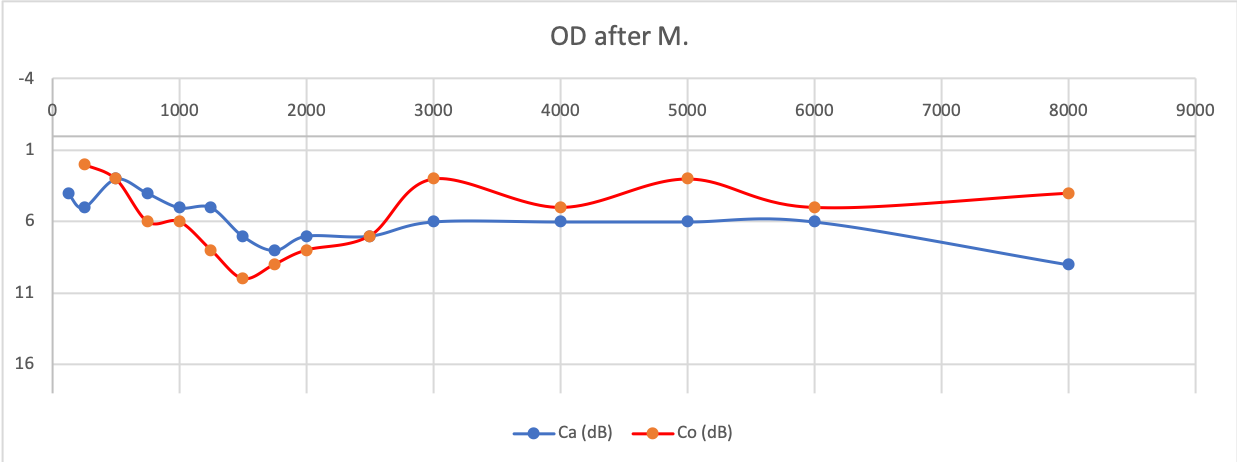
\includegraphics[width=1\linewidth]{images/clinique/od_before_m.png}
	\caption{Test d'écoute avant musicothérapie}
	\label{fig:odbeforemeyer}
\end{figure}
	\begin{figure}
	\centering
	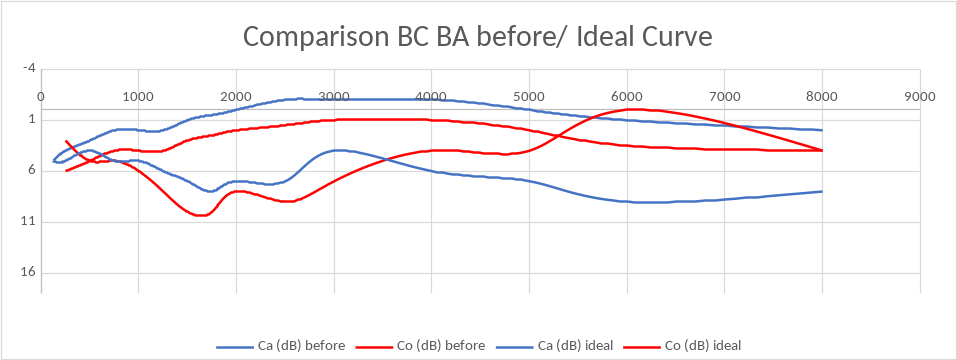
\includegraphics[width=1\linewidth]{images/clinique/comparison_bc_ba_before_vs_ideal_curve_meyer.png}
	\caption[Comparaison avec la courbe idéale]{Comparaison avant
		musicothérapie des
		courbes  avec la courbe idéale}
	\label{fig:comparisonbcbabeforevsidealcurvemeyer}
\end{figure}


\textbf{Déroulement général} :
Ayant le choix devant un grand instrumentarium,
le patient se dirige spontanément vers le piano, et très vite
l'\textit{émotion} monte: il pense à son père qui en jouait et qui
s'énervait contre lui, enfant essayant d'en
jouer. Il n'a jamais pris de cours, tapote avec un seul doigt et \textit{se considère comme
	amusica}l. Il essaie ensuite le piano-orgue  électrique: les \textit{sons bas}
lui procurent un énorme plaisir mais il n'ose pas enfoncer les touches
complètement car c'est trop fort, dit-il; d'autre part, il
craint également les
\textit{sons hauts.}
Après un moment, la thérapeute lui suggère d'essayer avec deux doigts.
Il enclenche le mode ``choeur'' et les sons se font beaucoup
plus présents, plus forts, mais il les accepte. Puis il commence à essayer spontanément
avec les autres doigts et remarque,  en s'étonnant, qu'il se
dirige tout de même vers les sons
hauts. Il \textit{s'amuse} à mêler les différentes tessitures,
les hautes comme les basses.
Il enclenche le mode ``drums'' et part d'un\textit{ joyeux
	fou-rire}. Retour en enfance, dit-il.
Il \textit{se détend} et prend de plus en plus de plaisir à jouer, particulièrement  les sons élevés
sur la droite et avec la main droite, et fait
la remarque suivante très surprenante:
\textit{``Ich kann meine Gefühle mit der rechten Hand steuern!''
	``Je peux diriger mes sentiments avec ma main droite''.}
Son expression à ce moment précis de la séance est saisissante: il
est gaucher et se sent très à l'aise d'utiliser son autre
main,-- \textit{``Komisch''},  \textit{``Etrange''}, se fait-il
la réflexion, très surpris de sa réaction-- et c'est un événement
accueilli comme une vraie
découverte--\textit{``Entdeckung''} --.
Il ajoute de plus, très affirmatif, que les sentiments avec sa main
droite ne sont plus une affaire de tête. \textit{``Keine
	Kopfsache mehr'''}. Il veut expérimenter le contraire, fait
une inversion d'utilisation des mains pour s'en convaincre et tout redevient comme
avant, c.à.dire \textbf{non fluide et retour au contrôle
	mental},
``bloquant'', dit-il. En inversant à nouveau, il retrouve
détente et fluidité.
A la séance suivante, il aimerait pouvoir ressentir
les sons dans tout son corps et ce sont les\textit{ bols
	tibétains } qui lui
apporteront tranquillité et
énergie. Utiliser désormais sa main
droite avec confiance l'aide, à ses dires, à analyser les
situations dans lesquelles il se trouve.


Dans ce qui précède, nous avons mis quelques mots en italique soulignant des  points
importants qu'amè\-ne un suivi en musicothérapie: l'émotion qui surgit très
vite,
l'attention du patient complètement happé par les sons --qui l'ont
contraint à être dans "l'instant présent "" ou une forme de méditation, la joie
enfantine qui réémerge avec le rire, la détente et la découverte,
ses propres observations et réflexions.
Il y a une imbrication forte des cinq sens, accompagnée par l'émotionnel, le comportemental, la
mémoire, en bref tout le système limbique et l'aspect
physiologique et psychologique.

De manière plus précise, nous faisons le constat, dans ce cas
particulier,  de la relation main droite, oreille droite, écoute
à droite et du probable impact sur l'hémisphère gauche.
Evidemment, nous ne pouvons généraliser son cas, (peut-être dû au hasard ou aux circonstances) et 
n'émettre qu'une hypothèse
en mettant en relation la nécessité d'une stimulation au niveau du cortex préfrontal
gauche -- partie de l'hémisphère gauche que l'écoute avec
l'oreille droite inciterait (générerait) -- pour activer l'analyse et la
mise en perspective des situations.

Le but est de trouver ou
retrouver un équilibre, une forme d'harmonie ou d'homéostasie, ce qui corroborerait les
propos de T. Janssen, recueilli dans  \autocite {van_eersel_cerveau}, démontrant la gestion des 
émotions par
l'un et l'autre des 2 hémisphères, soit le droit,  gérant les désagréables
(réflexe de survie, ne devant néanmoins pas se prolonger au risque de
développement de pathologies)
et l'autre, le gauche --- plus récent en terme d'évolution ---  les
agréables, indispensables pour relativiser les situations.

\textbf{ Test d'écoute post -- musicothérapie:}



\begin{figure}[h]
	\centering
	
	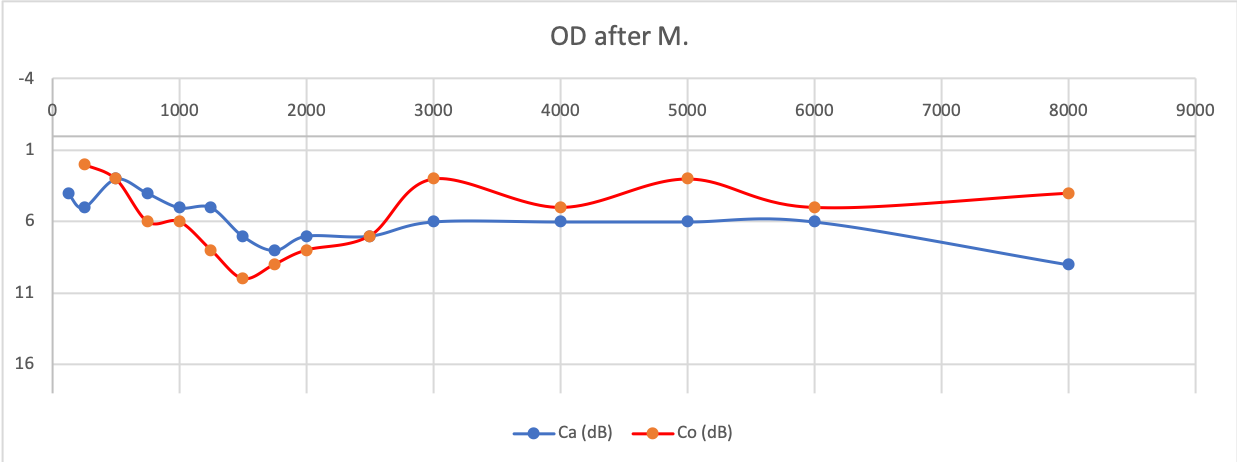
\includegraphics[width=1\linewidth]{images/clinique/od_after_m.png}
	\caption{Test d'écoute après la musicothérapie}
	\label{fig:odaftermeyer}
\end{figure}
Les relevés des trois tests correspondent à l'oreille droite.
Nous faisons les observations suivantes.
Avant musicothérapie: il n'existe pas d'harmonie dans le graphisme, les courbes ne suivant pas de 
parallélisme, la courbe osseuse  surplombe fortement l'aérienne 
à partir des fréquences de 3000 jusqu'à 8000 Hz.
Après musicothérapie:  les deux courbes se sont modifiées et tendent vers plus d'harmonie.
Elles se rejoignent, la courbe osseuse s'est abaissée vers l'aérienne.
 Plus précisément, la courbe aérienne, dans les
zones 2 et 3,  s'est modifiée, freinant sa
chute et se stabilisant à l'horizontal entre 3000 et 6000 Hz
avec des seuils de 5/6= 25 dB.
Dans les mêmes zones 2 et 3, la
courbe osseuse montait de 2500 à 6000 mais après traitement,
elle se modifie, se rapproche et abaisse ses seuils de
sensibilité en étant moins réactive aux sons de faible
intensité, donnée très positive: ainsi le très grand écart visuel dans la zone 3 s'amenuise beaucoup. Au 
niveau de cette
zone, une large progression dans
le domaine de la créativité semble s'élaborer. 

Avec les
seuils
de c. aérienne et c. osseuse des\textbf{ deux} oreilles (\textbf{droite et gauche)} en prenant toujours 
 la courbe idéale en référence, nous
constatons par contre les modifications chiffrées suivantes pré/post-traitement, à titre purement indicatif,
c. a.: 6,43/6,03 et c. o.: 6,25/6,85.
Ces chiffres, non utilisés pour l'étude mais issus de notre recherche, se sont nettement
modifiés et tendent vers
ceux dits ``idéaux''  qui équivalent aux environs de 1,3 pour
c. a. et 3,1 pour 
c. o. L'écart reste cependant très important. % 
%A
%des dégâts subis aux oreilles,dus aux  détonations d'armes manipulées en sa présence et
% sans protection, selon les dires du patient.
De plus, en observant la moyenne que nous obtiendrons de son oreille gauche et droite 
pré/post-traitement, (Cf. Etude 
clinique, Patient M. groupe GM), le
nombre de croisements n'aura ni augmenté ni diminué, ce qui ne nous donne 
aucun élément constructif.
 
En résumé, son écoute générale est très évolutive, elle se transforme avec un net profil d'amélioration, et 
plus particulièrement avec l'oreille
droite comme évoqué plus haut. L'ensemble est positif, tend vers un
rééquilibrage du tracé graphique des deux courbes. Le recueil des données du
questionnaire WHOQOL l'attestera et le confirmera.
Il reste cependant encore de larges perspectives de travail et d'amélioration.
Par conséquent, le test d'écoute est susceptible d'apporter des renseignements, lors
d'une analyse succincte pré/ post-traitement.


\chapter{Méthodologie} 

\section{Introduction}
 
\textbf{L'axe principal} porte sur l'observation par comparaison de la faculté d'écoute des 
patients lors de l'aboutissement d'une musicothérapie.
Prouver l'impact de la musicothérapie par des différences d'écoute pré/post - 
thérapie est l'objectif  recherché.
L'idée générale du test d'écoute est d'avoir un outil d'observation fiable, d'obtenir des repères 
dans le suivi et le processus musicothérapeutique, \enquote {avec un souci de rigueur dans une 
	perspective pragmatique et claire du point de vue clinique et institutionnel}\autocite[p. 
36]{vrait_musicotherapie_2018}. 
%C'est ce qui nous a motivé dans notre recherche. %Il est différent du 
%%test d'a
%Il serait intéressant pour la musicothérapie de prouver son impact par les différences d'écoute pré/post 
%- 
%thérapie.

\textbf{Les outils} sont constitués par  le test d'écoute Tomatis et le questionnaire WHOQOL sur la 
qualité de vie.


 %en gardant
 %leur indépendance par rapport à notre analyse, se déroulent simultanément, à
 %l'exception de la musicothérapie pour le groupe contrôle.
 
 
 \section{Description du setting}
 Nous allons
 d'abord exposer le cadre dans lequel nous avons fait ces tests et la
 population étudiée.
 
 La clinique privée (Privatklinik)
 de Meiringen (BE) est  principalement spécialisée en
 addictologie avec problèmes d'alcool et de toxicodépendance, couvrant aussi les aspects dépressifs
 et les
 burn-outs.
 Elle dispose d'une capacité de 195 lits, et le temps de séjour fluctue de 3 à 6 semaines ou plus, en
 fonction de la participation des assurances.
Actuellement, en plus de l'administration et l'intendance, les 33
 médecins et psychiatres sont
 accompagnés par 177
 soignants, dont des infirmiers psychiatriques, aide-infirmières, physio et
 ergothérapeutes,
 psychologues et intervenants en \textit{thérapies
 créatives}, comme l'art-thérapie, thérapie
 corporelle, zoothérapie (chien/cheval),  ateliers de créativité --
 bois et terre --,  les textiles et la\textbf{ musicothérapie} avec deux
 personnes, Regula Lehmann, musicothérapeute  à 90\%  à la clinique de Meiringen, et  l'auteure de ce 
 travail avec un remplacement fixe et régulier à 10 \%.
 
 \subsection{Consentement}
 Obtenu l'aval de la direction de la
 clinique pour cette étude,  le personnel soignant et l'ensemble des
 thérapeutes (ateliers, thérapies créatives, kynési--cyno--
 et hippothérapie) ont été  informés par un texte approuvé par la responsable des thérapies.
 Ce même texte, destiné aux
 patients, explique le projet de l'étude sur l'écoute, ainsi que la possible transformation de l'écoute,
 avec ou sans musicothérapie.
 Le consentement libre est validé par la signature du patient, après
 un court entretien avec lecture.\footnote{Cf. Annexe A. 10}
 %\footnote{musicothérapeute  à 90\%  à la clinique de Meiringen.}
 Comme le texte comportait des erreurs, il a été 
 corrigé après utilisation dans la Clinique.\footnote{Cf.Annexe A. 7}
 
  Le groupe témoin (GC) a été constitué de manière neutre, selon le souhait de participation à l'étude. 
 Les patients du groupe de musicothérapie (GM) 
 %ont reçu par ordonnance 
 % l'aval des médecins pour cette thérapie et 
 ont été planifiés et organisés grâce à l'aide de Regula Lehman.
 \subsection{Population}
 
 
 \textbf{ Pathologie des groupes}: Les patients ont été répartis en deux groupes sans différenciation de
 leur pathologie. Nous avons conscience d'avoir mélangé des symptomatologies qui
 toutefois paraissent
 sous-tendues par
 certains mécanismes
 similaires dont le
 noyau commun est une
 \textbf{difficulté de
 	régulation des
 	émotions},
 s'exprimant par une
 humeur négative: 
 troubles de la régulation émotionnelle
 dont le burn-out, les dépendances, la dépression.
 Il n'a pas été
 possible de différencier les pathologies, 
 diagnostic souvent incertain en début de séjour, raisons pour lesquelles elles
 se trouvent traitées ensemble.
 

 Chaque séance de musicothérapie a été suivie individuellement pendant 50 mn et uniquement par 
 l'auteure de ce 
 travail, lors des remplacements continus. Pour chaque test d'écoute, il en a été de même.
 
 
 
 L'\textbf{échantillonnage} -- fortement conditionné par les contraintes
 institutionnelles, comme les interruptions prématurées de séjour, les rendez-vous
 médicaux superposés, l'impossibilité de participation physique et/ou
 psychique,
 %les remplacements disparates et hétéroclites de ma
 %collègue,
 -- s'est réduit à un nombre limité de
 patients.
 Une autre contrainte de nature extra -- institutionnelle allant dans le
 même sens était dû à l'éloignement géographique de l'auteure: Genève/Meiringen.
 D'autre part, les conditions de l'étude à respecter, 
 à savoir la possibilité de procéder à la \textbf{ comparaison pré/ post -- thérapie} avec tests et 
 questionnaires, a eu un impact 
 certain sur le nombre de patients à analyser. 
 Nous avons fait, en plus des tests présentés, 18  tests  
 inutilisables car sans comparaison possible en fin de séjour.
 

 
  \textbf{Nous avons explicité trois cas par groupe  et mis à leur suite les autres avec le résumé des 
 résultats 
 sous la forme de tableaux}.
 
 
 
% L'autre option aurait été de supprimer les questionnaires, et de ne tenir compte que des test d'écoute,
% mais 
 %Ce sont les raisons pour lesquelles nous avons présenté un  nombre d'exemples  pour obtenir
% une parité avec les tests d'écoute pour la
 %\textbf{corrélation test d'écoute et questionnaire}.
 


%Les patients ont répondu aux questionnaires (le WHOQOL), réalisés en parallèle, pour obtenir 
%confirmation ou infirmation d'une modification de leur écoute en relation avec leur état psychique.


%\textbf{Résultats:} l'analyse de l'observation portant sur la transformation de l'écoute a montré une 
%positive et importante modification par comparaison pré/post traitement pour le groupe de 
%musicothérapie en relation avec le questionnaire WHOQOL. Pour le groupe contrôle, la transformation 
%était quasi inexistante et le questionnaire s'est révélé négatif.


%\textbf{Conclusions:} La musicothérapie a eu un impact positif sur la transformation de l'écoute, 
%corrélée 
%à l'état psychique, constatant une différence notable entre les deux groupes.


%\textbf{Remarque importante:} le nombre final de tests d'écoute corrélés aux questionnaires sera 
%inférieur à celui que l'on avait  planifié, réduisant considérablement la présentation des cas de ce travail. 
%en raison principalement
%'a pas pu être objective, 
%Due  principalement 
%à un manque important de questionnaires et  de séjours abrégés, la récolte des valeurs ne s'est 
%pas déroulée tel que projetée. 
%Le nombre de tests d'écoute n'ayant pas pu avoir lieu 
%en fin de thérapie, surtout en raison de séjours abrégés de patients a été moindre.
%Toutefois, il a été possible de recueillir des considérations allant dans le sens des questions de 
%recherche et d'étayer des résultats. Ce travail oscillera donc plus vers le qualitatif que le quantitatif, en 
%ayant tout à fait conscience des compétences scientifiques qu'un tel travail aurait exigé.



\section{Matériel}
\textbf{Outils de collecte de données: tests et questionnaires: }
Voici le matériel qui nous permettra de procéder à l'étude, avec une table et deux chaises.
\begin{enumerate}
	\item l'appareil
	test Hearing, les écouteurs pour calculer la courbe  aérienne et le vibrateur pour l'osseux, un crayon, 
	deux
	feutres (rouge et bleu), une feuille avec la grille de fréquences à
	remplir.
% des graphiques de courbes d'écoute permettent de 
%synthétiser des différences pré/post traitement 
%avec 15 patients répartis en 2 groupes de même type de pathologie 
%sur la qualité de vie. 
%les deux qualitatifs et quantitatifs.

	\item le test-questionnaire, le WHOQOL: 
les deux feuilles de questionnaires placées sur une table à l'entrée de la salle de musicothérapie.
\end{enumerate}
\begin{figure}
	\centering
	\includegraphics[width=1\linewidth]{images/testecoute.jpg}
	\caption[Appareil test écoute]{Matériel du test d'écoute, écouteurs, vibrateur et micro}
	
	\label{appareiltestecoute}
\end{figure}

\subsection *{Le test d'écoute}
Le test d'écoute détecte la manière de recevoir
l'information.
Nous obtenons une
\textbf{représentation graphique} générale des courbes de l'écoute
(équilibre, symétrie, harmonie) à partir des seuils d'écoute
calculés selon les fréquences et le volume que le sujet entend.
%avec des zones à lire et interpréter.
A cet effet, nous utiliserons l'appareil conçu à partir de 1950 par Alfred Tomatis, médecin
O. R. L.: le Hearing Test, testant
l'écoute pré/post - thérapie
afin d'établir une comparaison.
%L'utilisation particulière du \textit{test de perception d'écoute de Tomatis}  est
%légitimée par sa facilité et  simplicité d'application, en dehors de
%son contexte thérapeutique.\footnote{Nous précisons qu'aucun support de la méthode conçue par
%	Tomatis n'interviendra pendant les séances de musicothérapie.}
Nous pourrons constater
s'il existe un changement dans l'écoute du sujet grâce au support graphique, tel un ``dessin'',
une image. %fournissant des critères d'analyse.

\subsection* {Le WHOQOL  - Bref}  
Le World Health 	Organisation Quality of Life Assessement  (Cf. Annexe A. 9.) 
est un test d'évaluation de la qualité de vie, issu du
programme de l'Organisation Mondiale de la Santé, l'OMS.
Ce questionnaire est réalisé en parallèle, rempli par
les patients eux-même à l'entrée de leur séjour en clinique et
à leur sortie, avec ou sans musicothérapie.
Il s'agit ici de la version courte  la plus récente (2004) du questionnaire
WHOQOL-100 datant de 1998.
L'utilisation de ce questionnaire a pour but d'avoir
une variable supplémentaire pour confirmer ou infirmer en
parallèle l'action supposée  de la musicothérapie sur une éventuelle
modification de l'écoute.
Il sert aussi à constater s'il y a une\textbf{ transformation psychique }du sujet,
(positive ou négative) et s'il existe ou non une \textbf{corrélation }de
résultats avec le test d'écoute.

\section{Méthode d'analyse}
Nous allons décrire la manière d'analyser et collecter les résultats du questionnaire et du test d'écoute 
avec 13 patients répartis en 2 groupes de même type de pathologie (difficulté de régulation des 
émotions), l'un expérimental avec musicothérapie au nombre de 6 (GM) et l'autre, le groupe témoin au 
nombre 
de 7 (GC).
\subsection*{WHOQOL}
L'estimation se fait à partir d'une échelle
d'auto-évaluation subjective avec 26 questions courtes
dont un item concernant la qualité de vie globale
auto-évaluée par le sujet, un item évaluant la santé générale perçue
et les 24 autres se répartissent selon les 4 domaines suivants: physique, psychologique, relations 
sociales et environnement.
\begin{enumerate}
	\item  Le domaine de la perception physique (7 items) comprend l' activité quotidienne// la dépendance 
	et/ou l'assistance médicale// la fatigabilité, l'énergie//la mobilité// la douleur// le sommeil// la capacité 
	de travail//
	\item Le domaine psychologique (6 items):  image de soi, apparence// ressentis positifs et négatifs// 
	estime de soi// spiritualité, croyances personnelles, religion// mémoire et concentration, apprentissage, 
	pensée.
	\item Le domaine des relations sociales (3 items) : relations personnelles// soutien social// vie sexuelle.
	\item Le domaine de l'environnement (8 items) :
	l'environnement domestique et physique
	(pollution, bruit, trafic, climat)// la
	situation financière//  la liberté, la
	sécurité physique et morale//
	l'accessibilité et qualité de la santé// les
	opportunités de détente, loisirs, accès aux
	informations// logement et transport//
\end{enumerate}
Les questions varient selon sa propre perception, telle la satisfaction
au sujet de son  sommeil, de sa vie relationelle, sexuelle, de
l'opinion que l'on a sur soi, ou si le patient éprouve souvent des sentiments négatifs
et s'il a assez d'énergie dans la vie de tous les jours.
Le patient le remplit sans aide du
thérapeute lors de chaque test
d'écoute.

La cotation se fait sur 4 types d'échelles de réponses en 5 points (de 1 à 5)
permettant l'évaluation de l'intensité, la fréquence, la capacité.
Les résultats et les chiffres obtenus  sont calculés à partir de la moyenne des 4
domaines, pré -- et post -- traitement.
%est calculée pour chaque patient, à partir des scores
%des 4 domaines.
%Les chiffres ont été obtenus à partir des 4
%domaines, avec le pré/post-séjour.

\subsection*{Test d'Ecoute }
%avec comparatif pré/post-thérapie : données et résultats
Des graphiques de courbes d'écoute permettent  de synthétiser les différences et visualiser les 
moyennes oreille droite et oreille gauche pré/post 
traitement des 
deux groupes. Chaque test d'écoute  apparaitra transposé  sous forme de support informatique.
 La juxtaposition des seuils des deux oreilles nous permettent d'obtenir la moyenne de la 
 modification en allant du 
 premier au second test.
 % \textbf{moyenne} \textbf{des seuils
 %	auditifs de la courbe aérienne} de l'oreille \textbf{droite} et de
% l'oreille \textbf{gauche} de \textbf{chaque patient}:
% \item la \textbf{moyenne} \textbf{des seuils
 %	auditifs de la courbe osseuse} de l'oreille \textbf{droite} et de
 %l'oreille \textbf{gauche} de \textbf{chaque patient}
 
%une forme relevant clairement les courbes par des lignes 
%scannnon pas comme  les relevés à la main telle la  
%Fig. 8.1.
%  Les différentes moyennes des courbes et des  seuils.  Nous avons représenté  %Il s'agit ainsi d'une 
%%étude mixant le \textbf{quantitatif  et le
%	qualitatif}.
En procédant toujours en amont et en aval, --- pré/post-thérapie ---, nous
obtenons:
 %par \textbf{comparaison graphique des différentes
%	courbes}: 

\begin{enumerate}
	\item   les \textbf{seuils}  --moyenne
	représentée sous forme de la  \textbf{courbe aérienne}
	\item   les \textbf{seuils} --moyenne
	représentée sous forme de la \textbf{courbe osseuse}
\end{enumerate}

Pour procéder à la collecte des données, nous avons fait 
\begin{enumerate}
		
		\item la \textbf{comparaison des graphiques des différentes courbes}: allure générale, symétrie, 
		équilibre , en répondant à la question suivante:  
		Est-ce que la courbe a bougé, y a-t-il eu une modification? : réponse  positive ou négative.
		
	\item \textbf{les seuils: }
	Où se dirigent-ils ? 
	en observant le déplacement de leur direction,
	
	-   vers le haut, vers 0 dB : oui : positif ; on parle de relèvement des seuils.
	
	
	-   vers le bas du graphique: non: négatif: on parle d' abaissement des seuils.
	Lors de la passation du test, on remarque dans ce cas, que l'on doit augmenter sensiblement le 
	volume.
	%Indication technique: en sachant que lors de la 
%	passation du 
%	test, le volume est 
%	sensiblement augmenté.
	% donc   le 
	%volume doit être augmenté.
	
	%
	\item le \textbf{nombre de croisements entre courbe aérienne et courbe osseuse}
%	décompte
\end{enumerate}.
%Ainsi, après avoir
%fait une comparaison des dessins des différentes courbes et
%décompté le nombre des croisements, l'ensemble des résultats a été analysé et comparé, puis mis en 
%corrélation avec ceux du\textbf{
%	WHO QOL}.
 \subsection*{Collecte des résultats} 
Qu'il s'agisse des tests ou des questionnaires, nous avons choisi de façon originale et personnelle de
simplifier les résultats sous forme 
mathématique:  \textbf{ $+$, $=$, $-$ } avec les significations suivantes.


\textbf { Les test d'écoute: } 


Avec  le graphique des courbes:
\begin{enumerate}
	\item$+$   : amélioration, modification;  rapprochement significatif à la courbe dite idéale.
	\item$=$   : amélioration insignifiante, correspond à : $+/-$, (si c.a. $ + $ et c.o. $-$, ou vice-versa).
	
	\item$-$   : pas d'amélioration et pas/trop peu  de modification, inversion
	des courbes (c.o. supérieure à c.a.).
	
	Avec les \textbf{croisements}, les chiffres des tests pré/post
	nous permettent d'obtenir une comparaison:
	\item $+$ : plus petit est le nombre, meilleur est le résultat, ce qui correspond à un signe positif : $+$.
	\item$-$   : plus grand est le nombre, ce sera un signe négatif: $-$.
\end{enumerate}

\textbf{Le questionnaire WHOQOL:} 	
\begin{enumerate}
\item$+$  :  le score chiffré  en fin de séjour est plus élevé
que celui du
pré-séjour, le résultat final obtenu est considéré comme
positif et sera relevé  avec le signe : "+". 
\item $-$ : le score est plus bas et considéré comme négatif : "-"  
\item$=$ : le score pareil, sans changement,  comme avant le séjour, et reconnu sous le signe :  "=" .

Ensuite, pour créer le lien et la corrélation entre test écoute et questionnaire WHO QOL, nous ferons la 
somme finale des résultats des signes pour chacun afin de les comparer.
\end{enumerate}


  \clearpage
\section{Design de l'étude}




\begin{figure}%[hb]
	\centering
	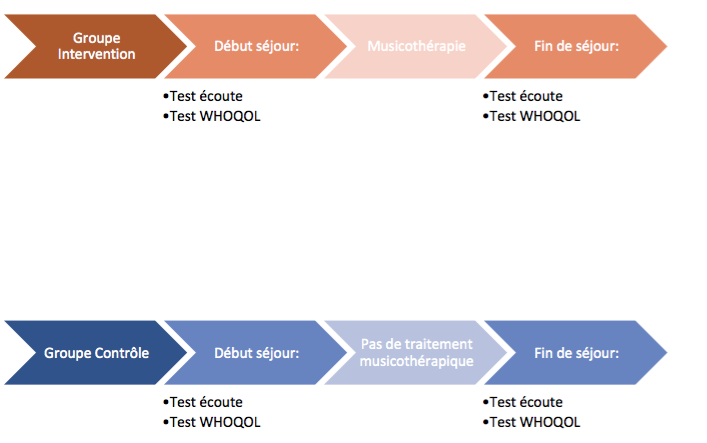
\includegraphics[width=1\linewidth]{images/Groupecontrole.png}
	\caption[Schéma du déroulement]{Déroulement de l'étude avec GM et GC}
	
	%\label{groupecontroleimage1}
\end{figure}

\textbf{L'étude} est
réalisée en fonction des séjours variables des patients, à l'aide de tests et questionnaires appliqués en 
début
et fin de séjour.

\textbf{Procédure}: chaque participant du groupe GM et GC va faire  un
test et remplir un questionnaire  WHOQOL en entrée et en sortie de
clinique  après environ 4 semaines, (GM ayant suivi une musicothérapie active et/ou réceptive 1x par
semaine:  comme signalé, le type de musicothérapie n'était pas imposé).
Chaque test d'écoute dure
70 à 90 minutes, fait 2x (pré/post-thérapie) et
suivi du questionnaire WHOQOL (2x10') rempli par le
patient lui-même.
Pour chaque patient : 2 tests d'écoute et 2 
questionnaires WQ 
remplis. Le critère d'exclusion: les patients n'ayant pas fait les deux tests d'écoute et pas répondu aux 
deux 
questionnaires ont été exclus.
La  figure (Fig.4.2) décrit de manière succincte le déroulement de
l'étude. 

 \clearpage




% Sur \textbf{44 tests d'écoute} réalisés pour \textbf{GC et GM},
%nous avons décompté\textbf{ 26 tests} valides qui serviront de
%comparatif dont \textbf{12} (6x2) pour
%GM groupe de musicothérapie,
%et \textbf{14 tests d'écoute} (7x2) pour GC le groupe
%contrôle, 14 questionnaires remplis  (7x2) pour GC et 4 pour GM (2x2).



%Voilà la manière dont s'est déroulée cette étude.
%pour aller jusqu'au bout de ce que nous avions décidé au départ, 





%\textbf{Index courbe idéale aérienne et osseuse}:
%La moyenne chiffrée de la courbe aérienne: 1,3
%La moyenne chiffrée de la courbe osseuse: 3,11
%Remarque: nous n'avons pas pu ici montrer l'intégralité des tests d'écoute, mais ceux-ci se trouvent à 
%disposition sur demande et en toute confidentialité.
%Notons que nous avons évidemment fait l'ensemble de l'analyse.
%Nous présenton
%Nous allons entrer dans l'étude clinique.
 
% et avons donc hésité à le signaler mais nà ne plus prendre en 
%compte cette parallèle. L'étude aurait été tronquée.
% aà chaque fois après 
